\section{Data}
\label{sec:data}
The data were collected from the public part of the Hacker One website. From 35 public bounty programs, we collected the rewards received by security researchers (in US dollars), with their timestamps. Since HackerOne started its platform in December 2013, new programs have been launched roughly every two months, following an essentially memoryless Poisson process ($\lambda = 57$ days, $p < 0.001$ and $R^2 > 0.99$). Figure \ref{timeline}A shows the timeline of the 9 most active programs with at least 90 (rewarded) bug discoveries, as of February 15, 2016. When a new program is launched, we observe an initial peak (or within weeks after launch), which accounts for the majority of discoveries, suggesting a {\it windfall} effect. Following the initial surge of vulnerability discoveries, bounty awards become less frequent following a decay function with long-memory, following a robust power law decay $\sim t^{\alpha}$ with $\alpha = -0.40(4)$ ($p < 0.001$ and $R^2 = 0.79$) at the aggregate level and over all 35 bounty programs, with weekly binned time series of bug discoveries normalized by their initial value (see Figure \ref{timeline}B).\\


\begin{figure}[Ht]
\begin{center}
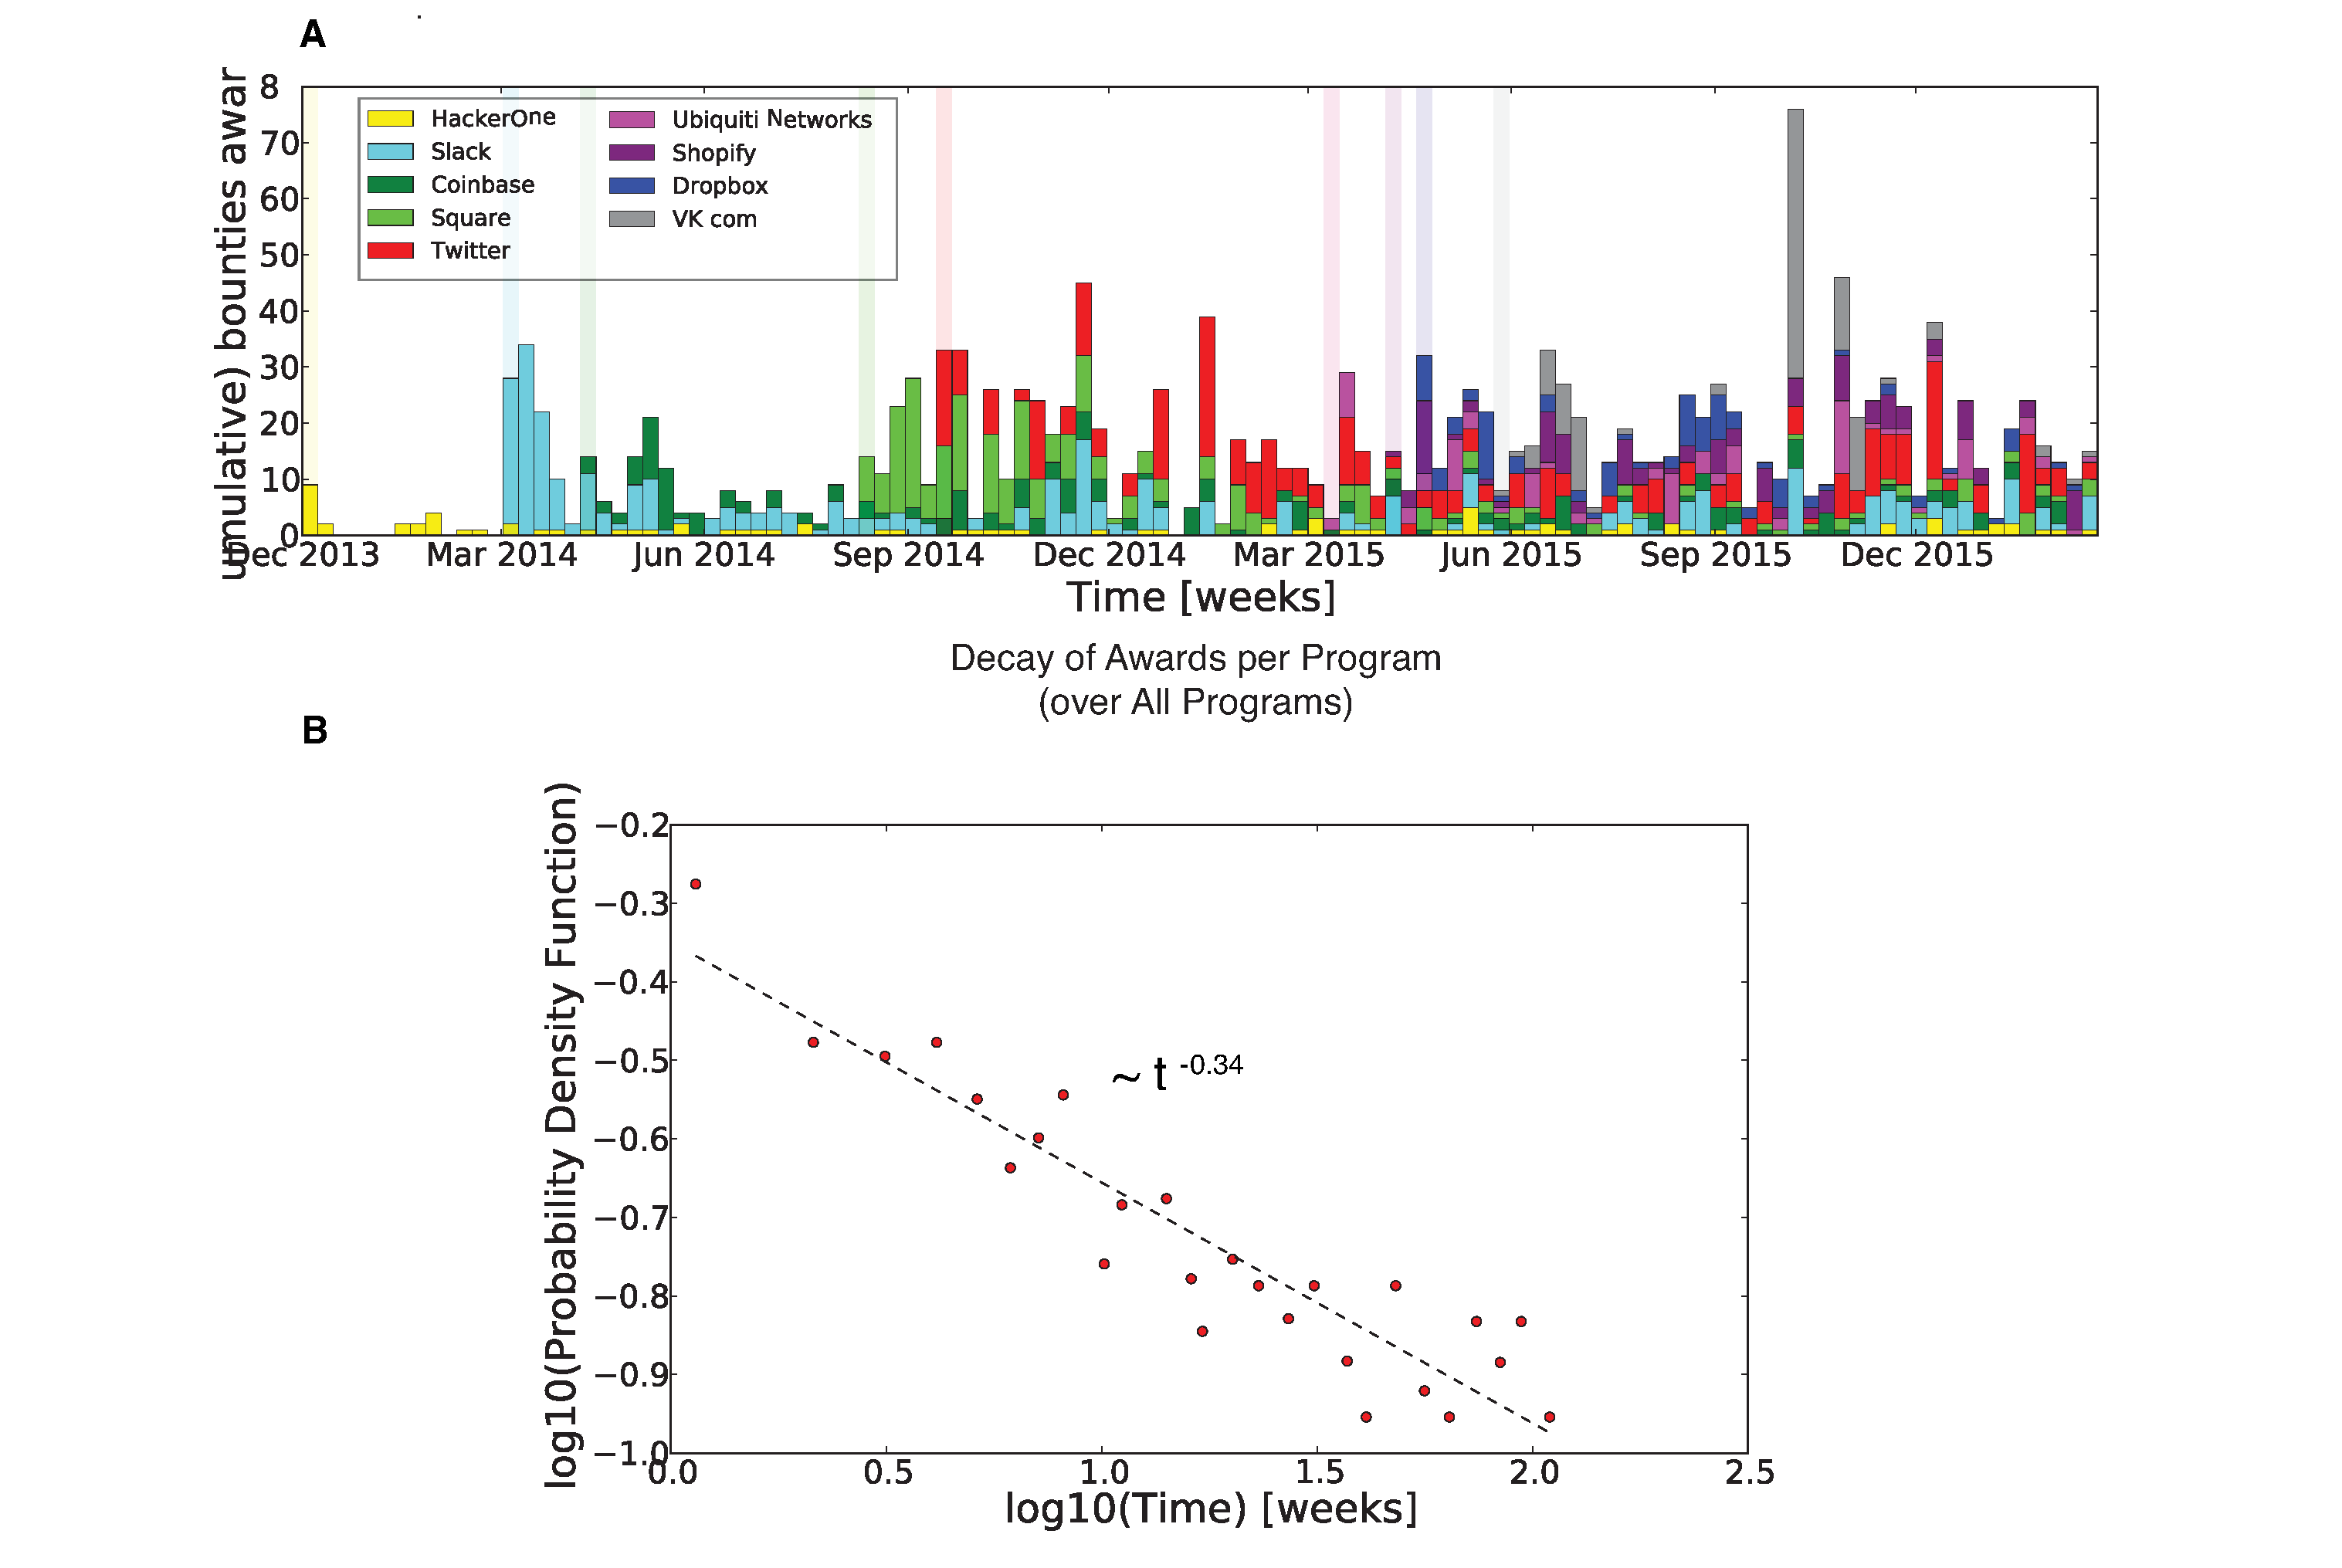
\includegraphics[width=13cm]{figures/timeline.eps}
\caption{{\bf A.} Weekly vulnerability discoveries for the 9 most active programs (with at least 90 bug discoveries as of February 15, 2016). The light colored vertical bars represent the start of the program, occurring when the first bounty is awarded. Most programs exhibit an initial shock (or shortly after the start of the program), followed by a decay of discoveries, which is characterized at the aggregate level by a long-memory process (panel {\bf B}) characterized by a power law decay $\sim t^{\alpha}$ with $\alpha = -0.40(4)$ ($p < 0.001$ and $R^2 = 0.79$). Each data point in the figure is the median of normalized vulnerability numbers of all 35 programs considered in this study.}
\label{timeline}
\end{center}
\end{figure}


The long-memory process of bug discovery following the launch of a bounty program we observe here, is reminiscent of human timing effects: When the program launches, it takes some time first for the researcher to be exposed to the new program (through the media and social media); Second for the researcher to find and submit bugs, and third for the organization managing the bug bounty program to assess the quality of each submission, and assign a proper reward. To account for all these delays, one may resort to priority queueing applied to humans: First, competing attention prevents immediate exposure to the news of a new program; Second, when security researchers get interested in a new program, they may still be actively searching bugs on other programs or performing other tasks, such as e.g., their regular job, leisure, family matters); Third, when subjected to a flow of bug submissions, security teams at organizations leading bounty programs assign priorities among submissions, and resolve them with human resources available at the time of submission. These delays are best rationalized by human timing contingencies, and moreover, by time as a scare, non-storable resource, which are known to generate long-memory responses of the form $\sim t^{-1.5}$ (in fully rational case) between the arrival and the execution of a task\cite{maillart2011quantification}. The observed much slower decay may result from the compound effect of multiple delays, such as those mentioned above. The initial burst of discoveries, followed by a long-memory decay may also result from the increasing difficulty associated with finding new bugs for each bounty program, as the most obvious vulnerabilities get uncovered first.  Since, we consider only the {\it time of discovery} as the moment when the validity of the bug submitted is acknowledged by the program manager, we are mostly blind to the human timing effects associated with the long-memory process observed on Figure \ref{timeline}B, including when submissions are made, but don't lead to a discovery associated with a monetary reward.\\

